\documentclass[a4paper, 12pt]{article}

\usepackage[margin=0.5in]{geometry}

% Packages for figure
\usepackage{float}
\usepackage{graphicx}
\graphicspath{{Image/}}
\usepackage{subfig}

%packages for reference
\usepackage[hidelinks]{hyperref}
\usepackage{url}




\begin{document}

	\tableofcontents
	\pagebreak
	\listoffigures
	\pagebreak
	\listoftables
	\pagebreak
	
	\section{Image}
	This is a sample document to illustrate how to insert image in a LaTex document. In this document we will illustrate different image insertion techniques.
	\subsection{Single Image}
	\begin{figure}[H]
		\centering
		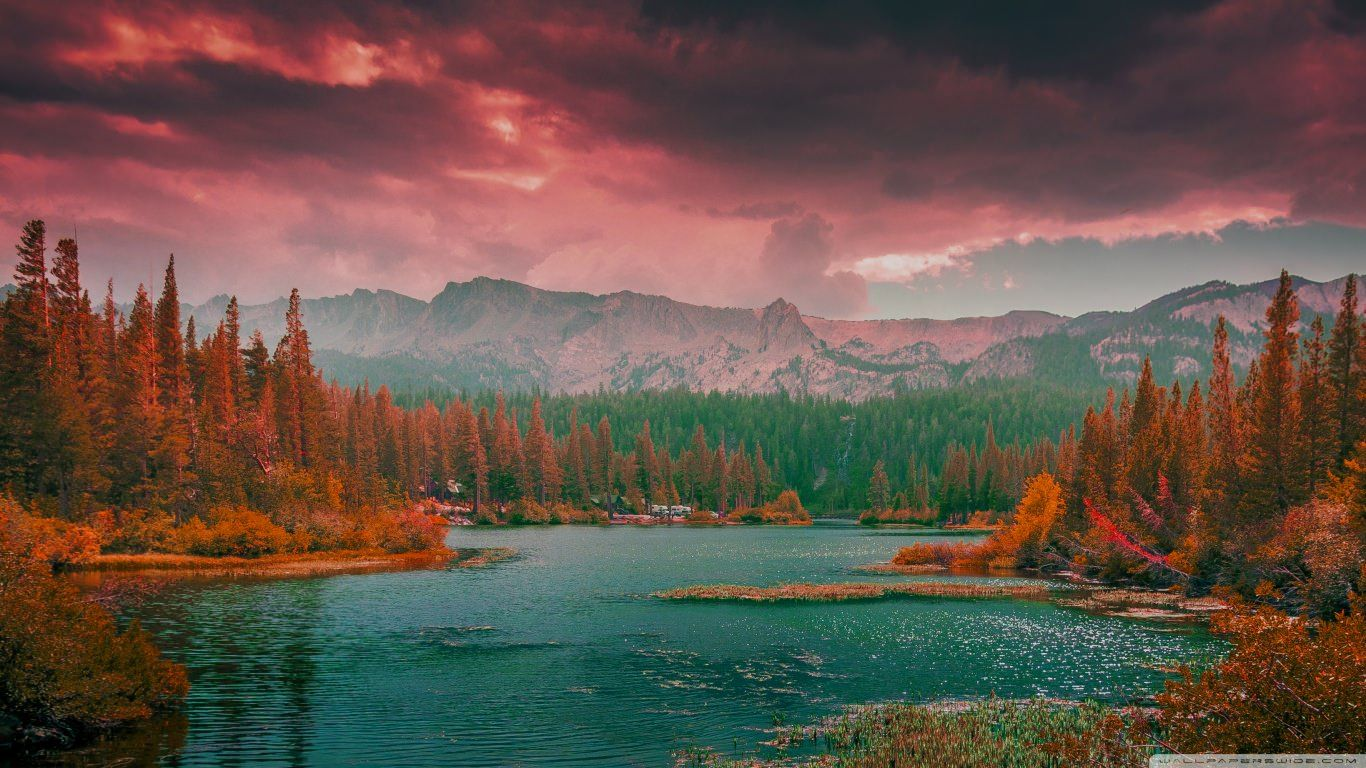
\includegraphics[scale=0.25]{two}
		\caption{Beautiful Picture of Water Body}
		\label{two}
	\end{figure}
	
	\subsection{Sub-Image}	
	Now in below we will show how to use subfigure. For this purpose we are using float(subfloat). Subfloat is very useful for placing subfigures at any desired position.
	
	\begin{figure}[H]
		\centering
  		\subfloat[Rural Picture]{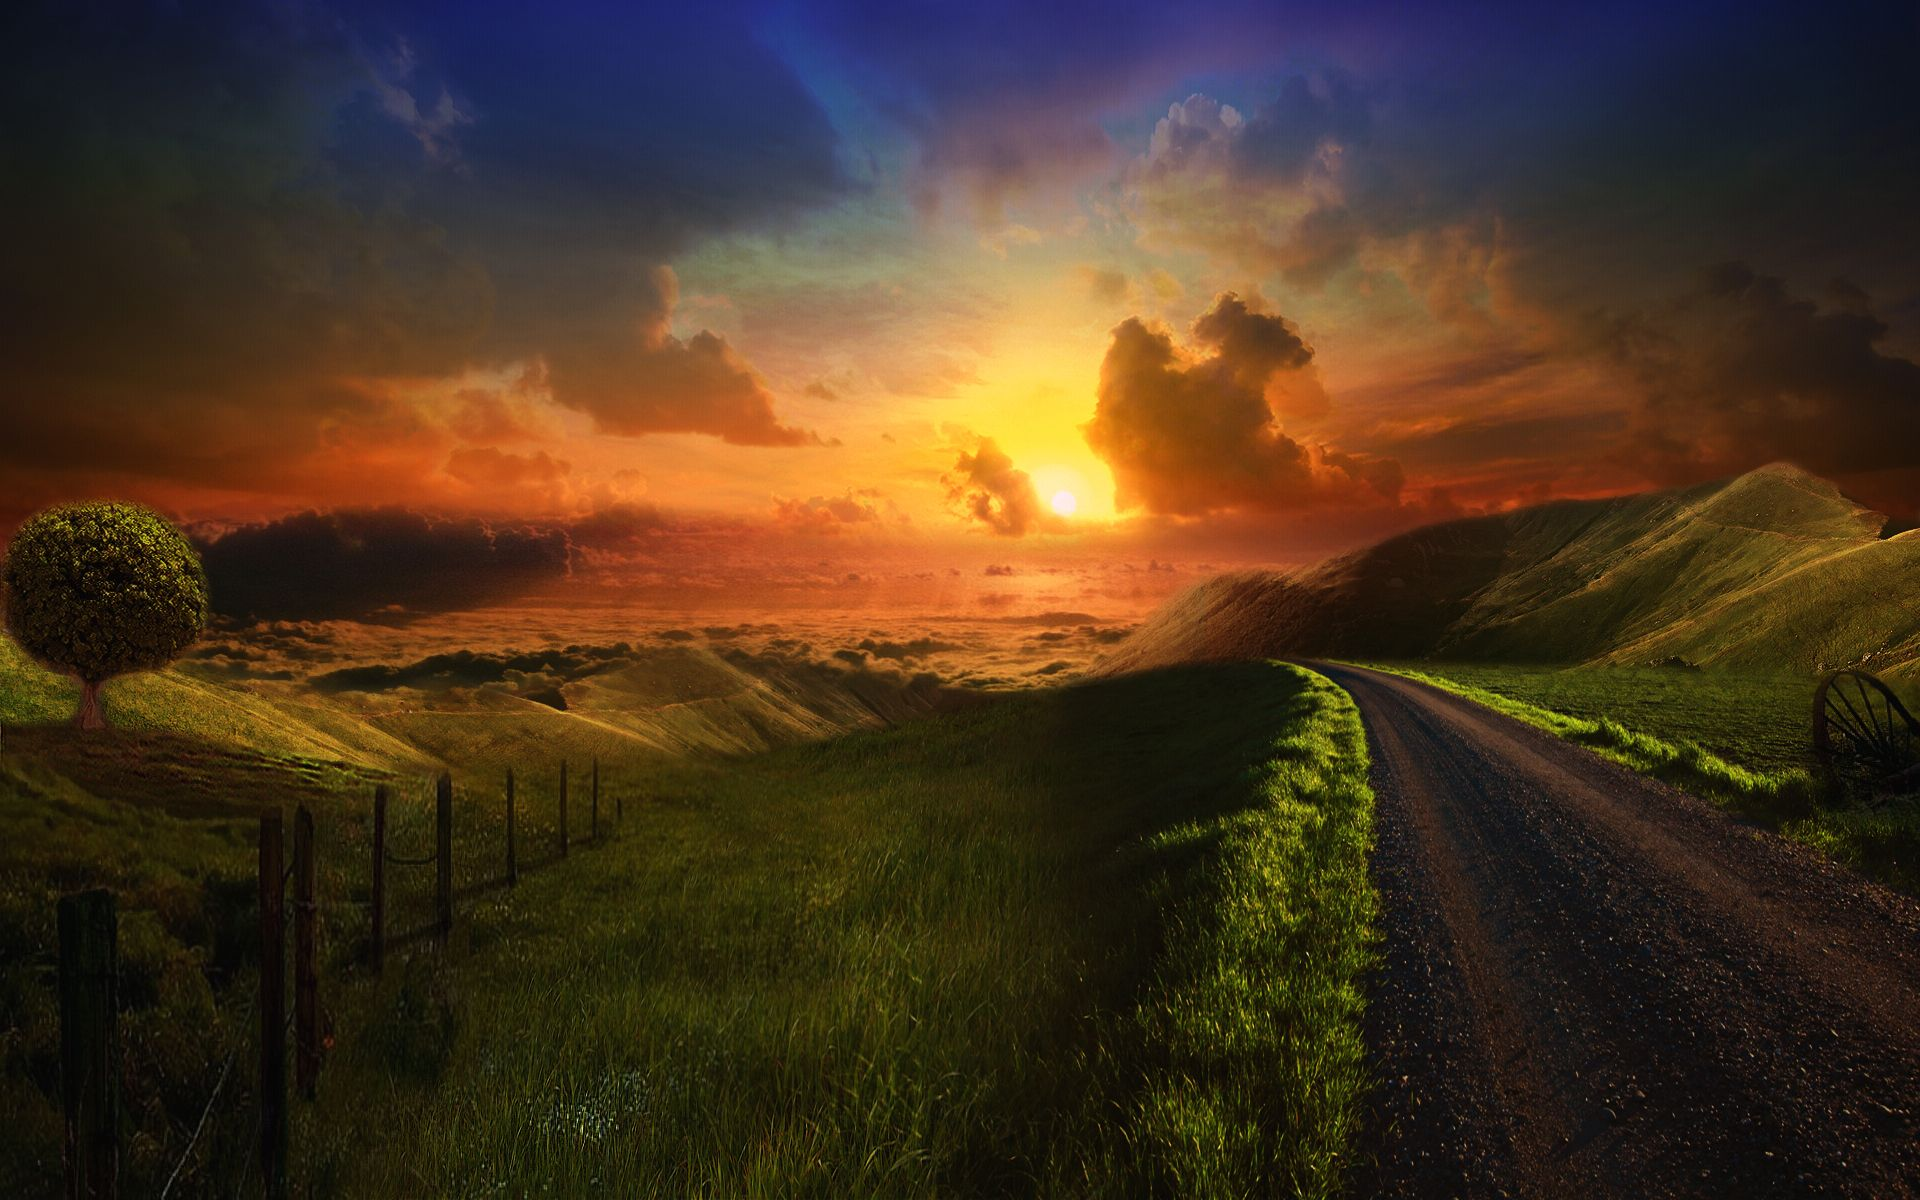
\includegraphics[width=0.4\textwidth, height=40mm]{one}\label{fig:one}}
  		\hfill	% This is to fill the space horizontally. Try removing it and see the effect
  		\subfloat[Urban Picture]{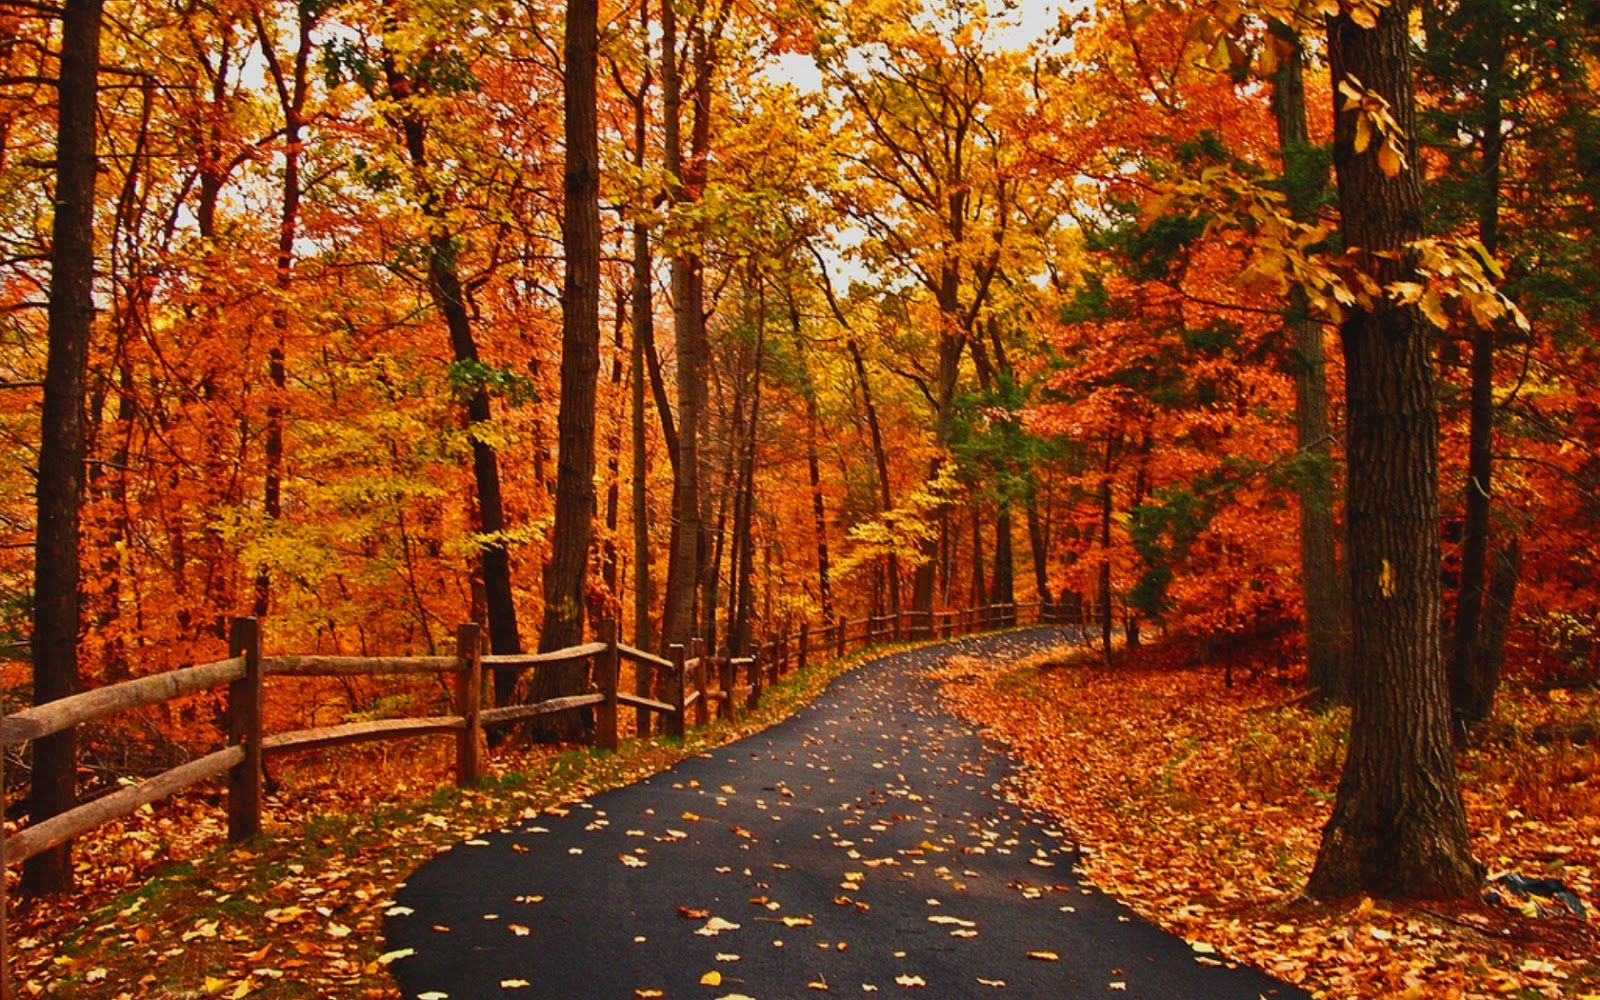
\includegraphics[width=0.4\textwidth, height=40mm]{three}\label{fig:three}}
  		\vspace{1cm}
  		\subfloat[Beautiful Sunset]{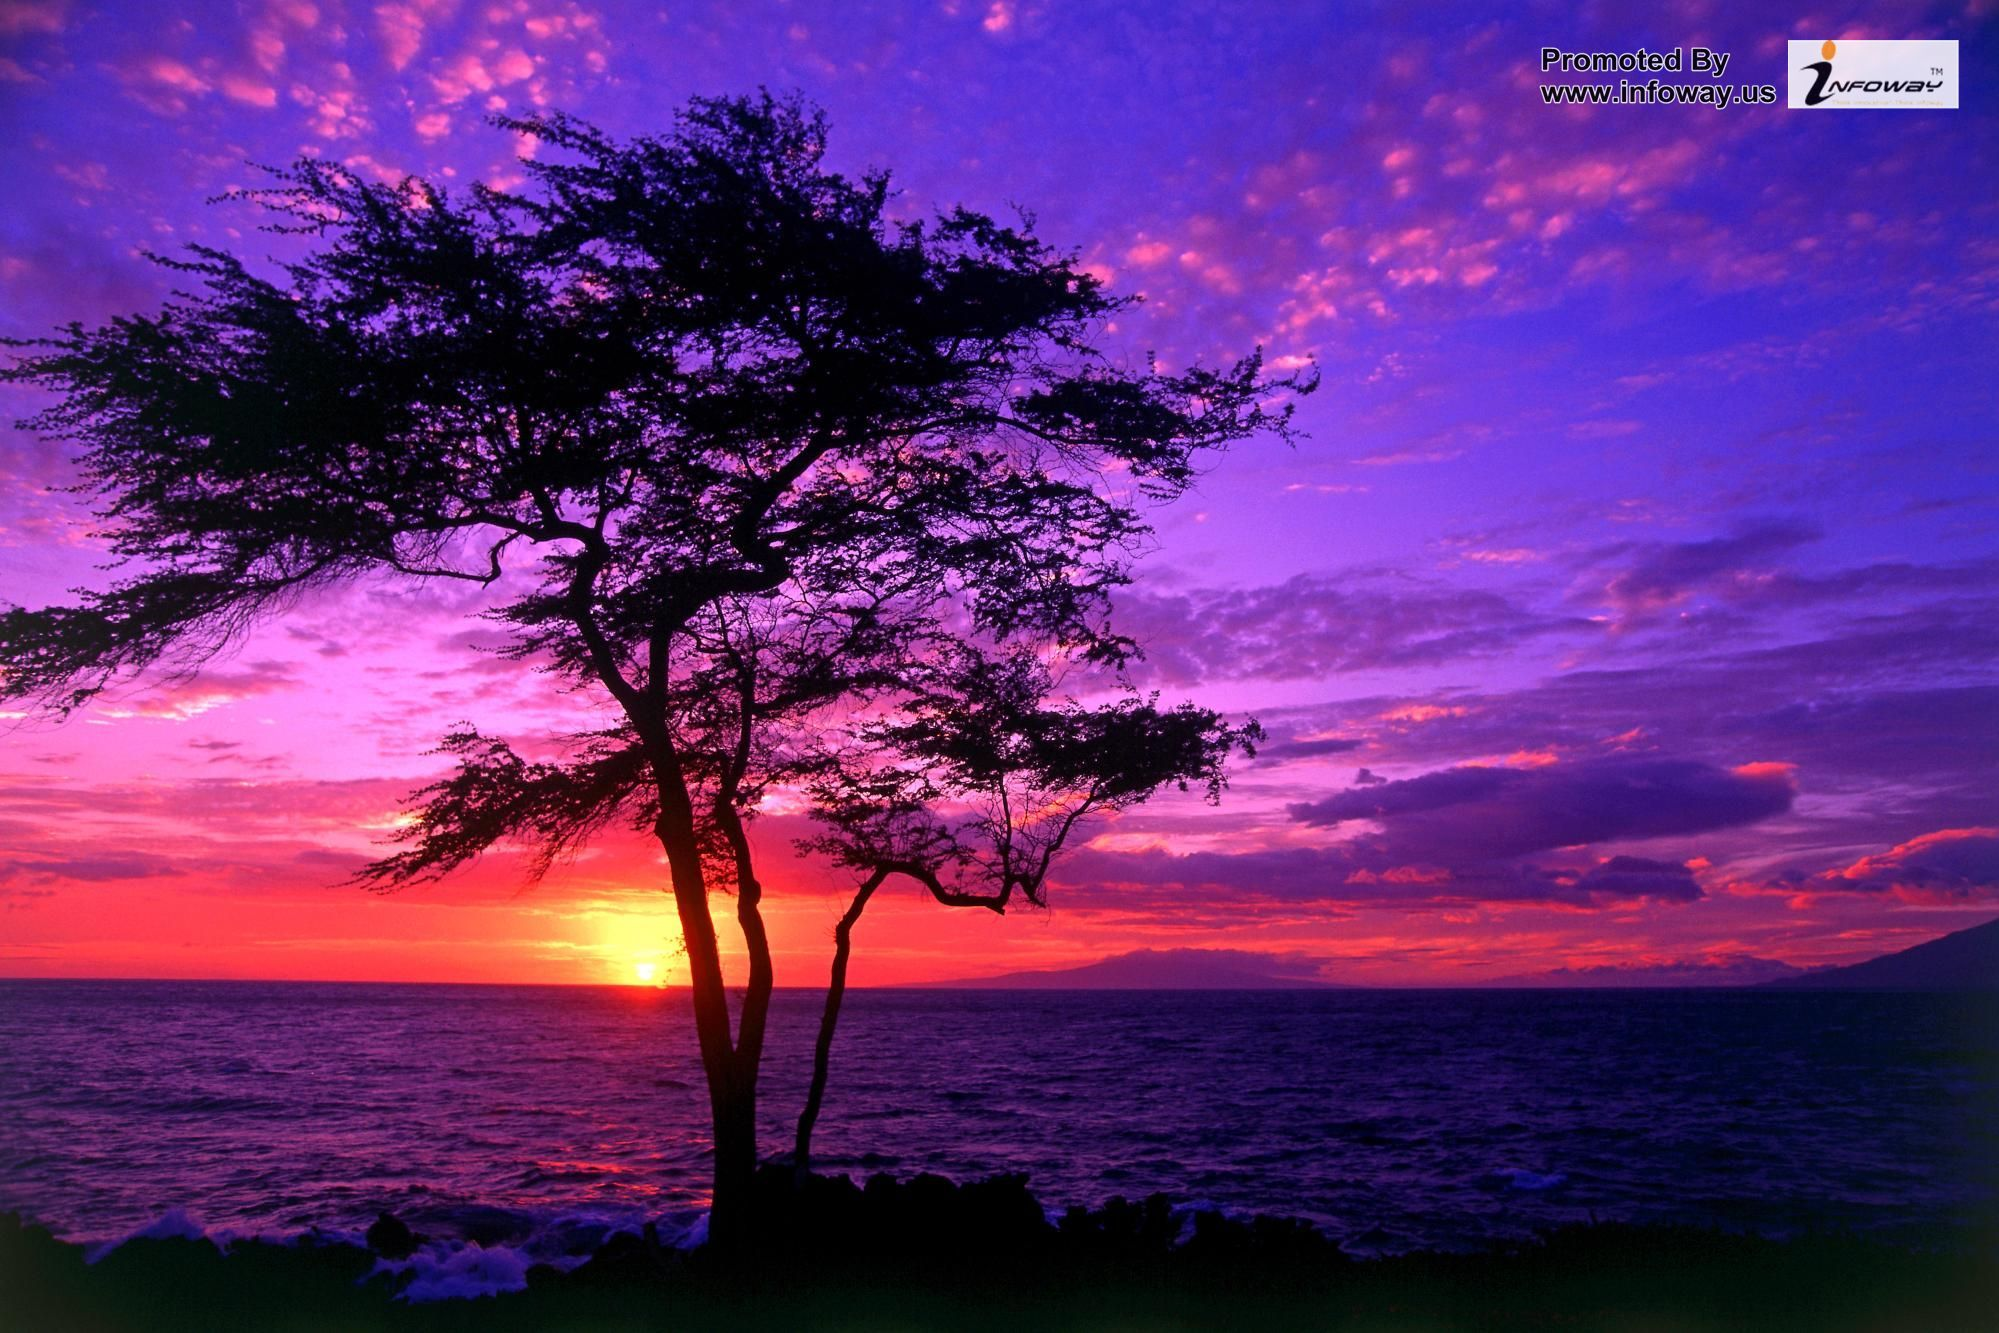
\includegraphics[width=0.4\textwidth, height=40mm]{four}\label{fig:four}}
  		\caption{Two different pictures of road and beautiful sunset}
  		\label{fig:effctofnoise}
	\end{figure}
	\pagebreak
	
	\section{Some Random Tables}
	\begin{table}[H]
		\label{tab:bayoldsummery}
		\centering
		\caption{Predefined word segmentation technique Summary}
		\begin{tabular}{ | c | c | }
			\hline
			Measures & Values \\
			\hline\hline
			Correctly Classified Instances & 68\%  \\ 
			Incorrectly Classified Instances & 32\%  \\  
 			Kappa statistic & 0.6 \\   
			Mean absolute error & 0.134 \\
			Root mean squared error & 0.318 \\
			Relative absolute error & 40.9848\% \\
			Root relative squared error & 77.7555 \% \\
			Total Number of Instances & 25  \\
			\hline
		\end{tabular}
	\end{table}	

	\begin{table}[H]
		\label{tab:baypropsummery}
		\centering
		\caption{Proposed word segmentation technique Summary}
		\begin{tabular}{ | c | c | }
			\hline
			Measures & Values \\
			\hline\hline
			Correctly Classified Instances & 76\%  \\ 
			Incorrectly Classified Instances & 24\%  \\  
 			Kappa statistic & 0.7 \\   
			Mean absolute error & 0.0963 \\
			Root mean squared error & 0.2933 \\
			Relative absolute error & 29.4411\% \\
			Root relative squared error & 71.6988 \% \\
			Total Number of Instances & 25  \\
			\hline
		\end{tabular}
	\end{table}	
	
	\begin{table}[H]
		\label{tab:bayoldconfusion}
		\centering
		\caption{Predefined word segmentation technique Confusion Matrix}
		\begin{tabular}{ | c | c | c | c | c | c | }
		\hline
		Classified as & A & B & C & D & E \\
		\hline\hline
		A = and & 4 & 0 & 0 & 0 & 1 \\
		B = in & 0 & 2 & 0 & 0 & 3 \\
		C = of & 0 & 4 & 0 & 1 & 0 \\
		D = the & 0 & 0 & 0 & 5 & 0 \\
		E = to  & 0 & 2 & 1 & 0 & 2 \\
		\hline
		\end{tabular}
	\end{table}
	
	\begin{table}[H]
		\label{tab:baypropconfusion}
		\centering
		\caption{Proposed word segmentation technique Confusion Matrix}
		\begin{tabular}{ | c | c | c | c | c | c | }
		\hline
		Classified as & A & B & C & D & E \\
		\hline\hline
		A = and & 4 & 1 & 0 & 0 & 0 \\
		B = in & 0 & 4 & 0 & 1 & 0 \\
		C = of & 0 & 3 & 1 & 1 & 0 \\
		D = the & 0 & 0 & 0 & 5 & 0 \\
		E = to  & 0 & 0 & 0 & 0 & 5 \\
		\hline
		\end{tabular}
	\end{table}
	
	
	\pagebreak
	
	This is to check wheather the references are working or not. My first reference is \cite{one}. The second one is \cite{jurafsky2000speech} and so on.\\
	
	Remember if you do not refer a particular entry in your bibliography it will note be shown in reference.\\
	
	There are many bibliography styles present to use and you can use any one of them. You can find them in online.
	
	\addcontentsline{toc}{section}{References} %This line is to make sure bibliography is present in table of centents
	\bibliographystyle{plain}
	\bibliography{reference}

\end{document}